% ----------------------------------------------------------
% Introdução (exemplo de capítulo sem numeração, mas presente no Sumário)
% ----------------------------------------------------------
\chapter[Introdução]{Introdução}
%\addcontentsline{toc}{chapter}{Introdução
% ----------------------------------------------------------

 A siderurgia é o ramo da metalurgia que se dedica à fabricação de ferro e aço  através do processamento do minério ferro, sucata, carbono, carvão e fundentes (\textit{e.g.} calcário e dolomita). Existem dois tipos de usinas siderúrgicas: a usina simples, que só utiliza como matéria prima o carvão mineral e a usina integrada, que utiliza tanto o carvão mineral como o carvão vegetal em sua produção (Figura \ref{fig:fluxogramaSiderurgia}).
 
  \begin{figure}[H]
	\centering
	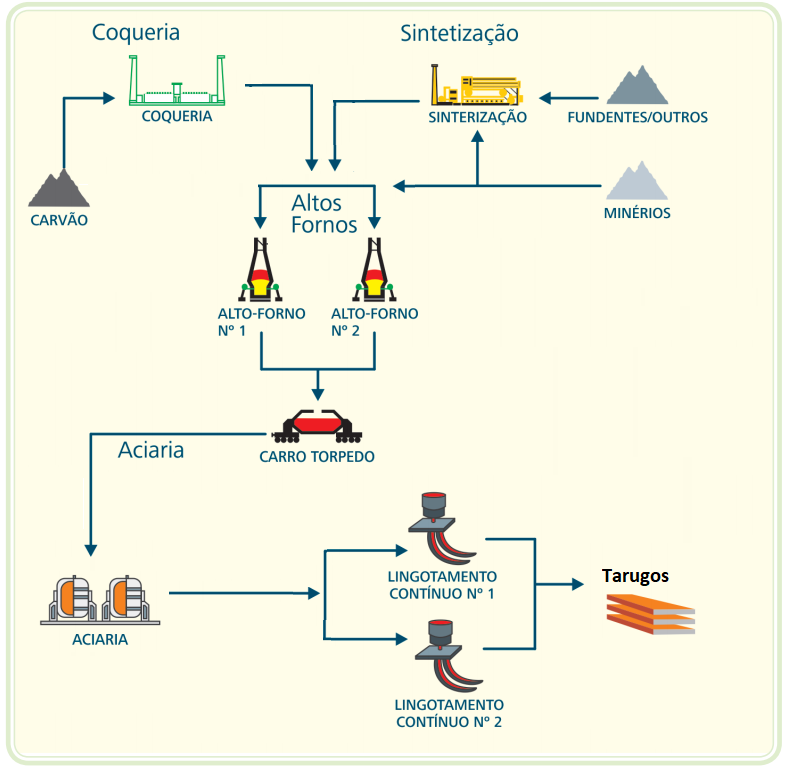
\includegraphics[width=0.6\linewidth]{figuras/Steel/fluxogramaSiderurgia.png}
	\caption{Processo siderúrgico}
	\legend{Fonte: \cite{silva2016siderurgia} }
	\label{fig:fluxogramaSiderurgia}
\end{figure}

 A primeira etapa do processo siderúrgico é a Coqueria. Nela, o minério de ferro é transformado em pelotas através do processo de Pelotização e o carvão mineral é destilado para obtenção do coque.
%
As usinas integradas incluem o processo de Sinterização, cujo intuito é produzir sínter por meio da aglomeração do minério de ferro, fundentes e finos de coque.

 O coque e o sínter são levados aos Alto-Fornos, cuja temperatura média de operação é de 1.500ºC. Dentro dos Alto-Fornos, o ferro se liquefaz e passa a ser chamado de ferro-gusa. Ele é levado à Aciaria por carros torpedos para refinamento através da queima das impurezas. Ainda na Aciaria, a oxidação de elementos como o carbono, silício, fósforo e enxofre transformam o ferro-gusa em aço líquido. Ele é então encaminhado para o Lingotamento Contínuo e, em processo de solidificação, é trabalhado mecanicamente e transformado em produtos como tarugos, bobinas, arames, etc \cite{aco}.

Na usina da Gerdau em Ouro Branco, o processo de lingotamento consiste no despejamento de uma panela com aproximadamente 224 toneladas de aço, a uma temperatura de cerca de 1550ºC, no distribuidor que precede o lingotamento em si como mostra a Figura \ref{fig:processLing}.
%
Este processo pode levar de horas a dias sem interrupção.
%
Cada batelada da panela é chamada de corrida.
%
No final de cada corrida, os tarugos são cortados na máquina Oxicorte, de modo que o tamanho é previamente definido de acordo com a necessidade do cliente, como identificado pelo número 5 na Figura \ref{fig:processLing}

 \begin{figure}[H]
	\centering
	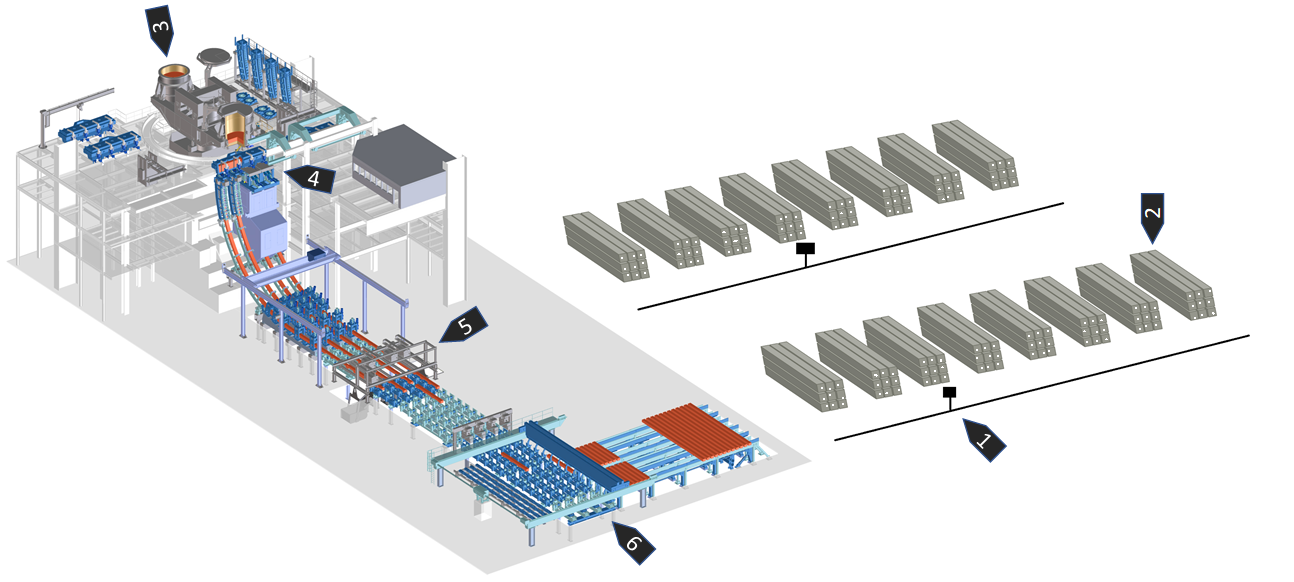
\includegraphics[width=1\linewidth]{figuras/Steel/process.png}
	\caption{Processo de lingotamento Contínuo de Tarugos}
	\legend{Fonte: \cite{freitas2013analise} }
	\begin{tabular}{r@{: }l r@{: }l}
        1 & Câmera Fotográfica & 4 & Molde \\
        2& Pilha de corridas & 5 & Máquina de Oxicorte \\
        3 & Panela de aço& 6 & Transferidor de tarugos \\
    \end{tabular}
	\label{fig:processLing}
\end{figure}

A etapa de solidificação ocorre de fora para dentro do veio
%
\footnote{\textit{Veio} é o nome que se dá ao conjunto formado pelo molde, a máquina Oxicorte e os rolos de extração e endireitadores. Quanto maior o número de veios mais produtiva é da máquina, porém mais complexo se torna seu controle.} 
%
em função do contato com as paredes refrigeradas do molde, aspersão de água em \textit{sprays} e perda de calor por radiação para o ambiente. Essa troca de calor faz com que o aço se solidifique gradativamente criando zonas onde o material pode ser encontrado ao mesmo tempo em seus estados sólido na parte exterior e líquido no interior (Figura \ref{fig:processLingSolid}).

\begin{figure}[H]
	\centering
	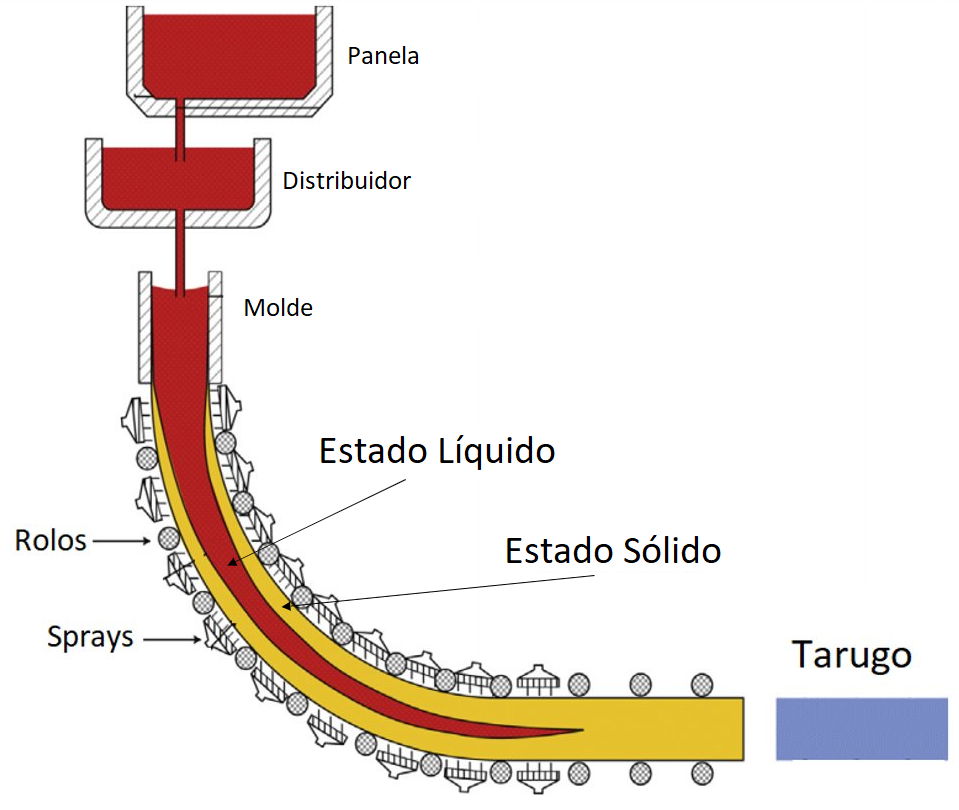
\includegraphics[width=0.6\linewidth]{figuras/Steel/estadoSolidoLiq.png}
	\caption{Estados do aço no processo de lingotamento contínuo}
	\legend{Fonte: \cite{YU201736}}
	\label{fig:processLingSolid}
\end{figure}

Os tamanhos dos cortes são feitos de acordo com a demanda do cliente. O número de tarugos depende do diâmetro das peças que podem ser de 130mm ou 160mm e do comprimento das mesmas que variam de 07 a 14m. Todas as peças de uma mesma corrida têm o mesmo diâmetro e comprimento. Após serem cortados, os tarugos são transportados para o despacho por uma ponte rolante a base de eletroímãs que suportam altas temperaturas e $27$ toneladas de carga (Figura \ref{fig:crane}). 

\begin{figure}[H]
	\centering
	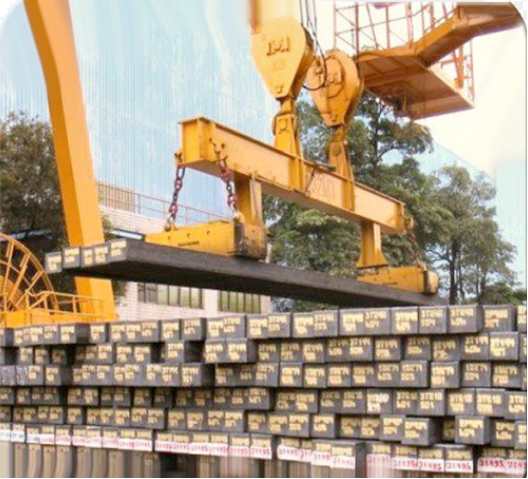
\includegraphics[width=0.5\linewidth]{figuras/Steel/ponte_rolante.png}
	\caption{Ponte Rolante}
	\legend{Fonte: \cite{ponte-rolante})}
	\label{fig:crane}
\end{figure}

Os tarugos vão para a zona de despacho a uma temperatura de aproximadamente 700ºC.
%
Após cerca de 20 horas a temperatura cai para $150~$ºC, adequada para a fixação das etiquetas de identificação dos tarugos.
%
Um jato de água é direcionado aos tarugos para acelerar o resfriamento como mostrado na Figura \ref{fig:despacho} com vazão constante apenas na parte frontal.
%
A eventual injeção de água no centro do tarugo pode empenar a peça, uma vez que a temperatura central do tarugo está mais quente que as extremidades.

Após o tempo necessário, o operador prega as etiquetas utilizando Silicone Acético Transparente, material comprovadamente aderente em altas temperaturas (Figura \ref{fig:barcode}).

\begin{figure}[H]
	\centering
	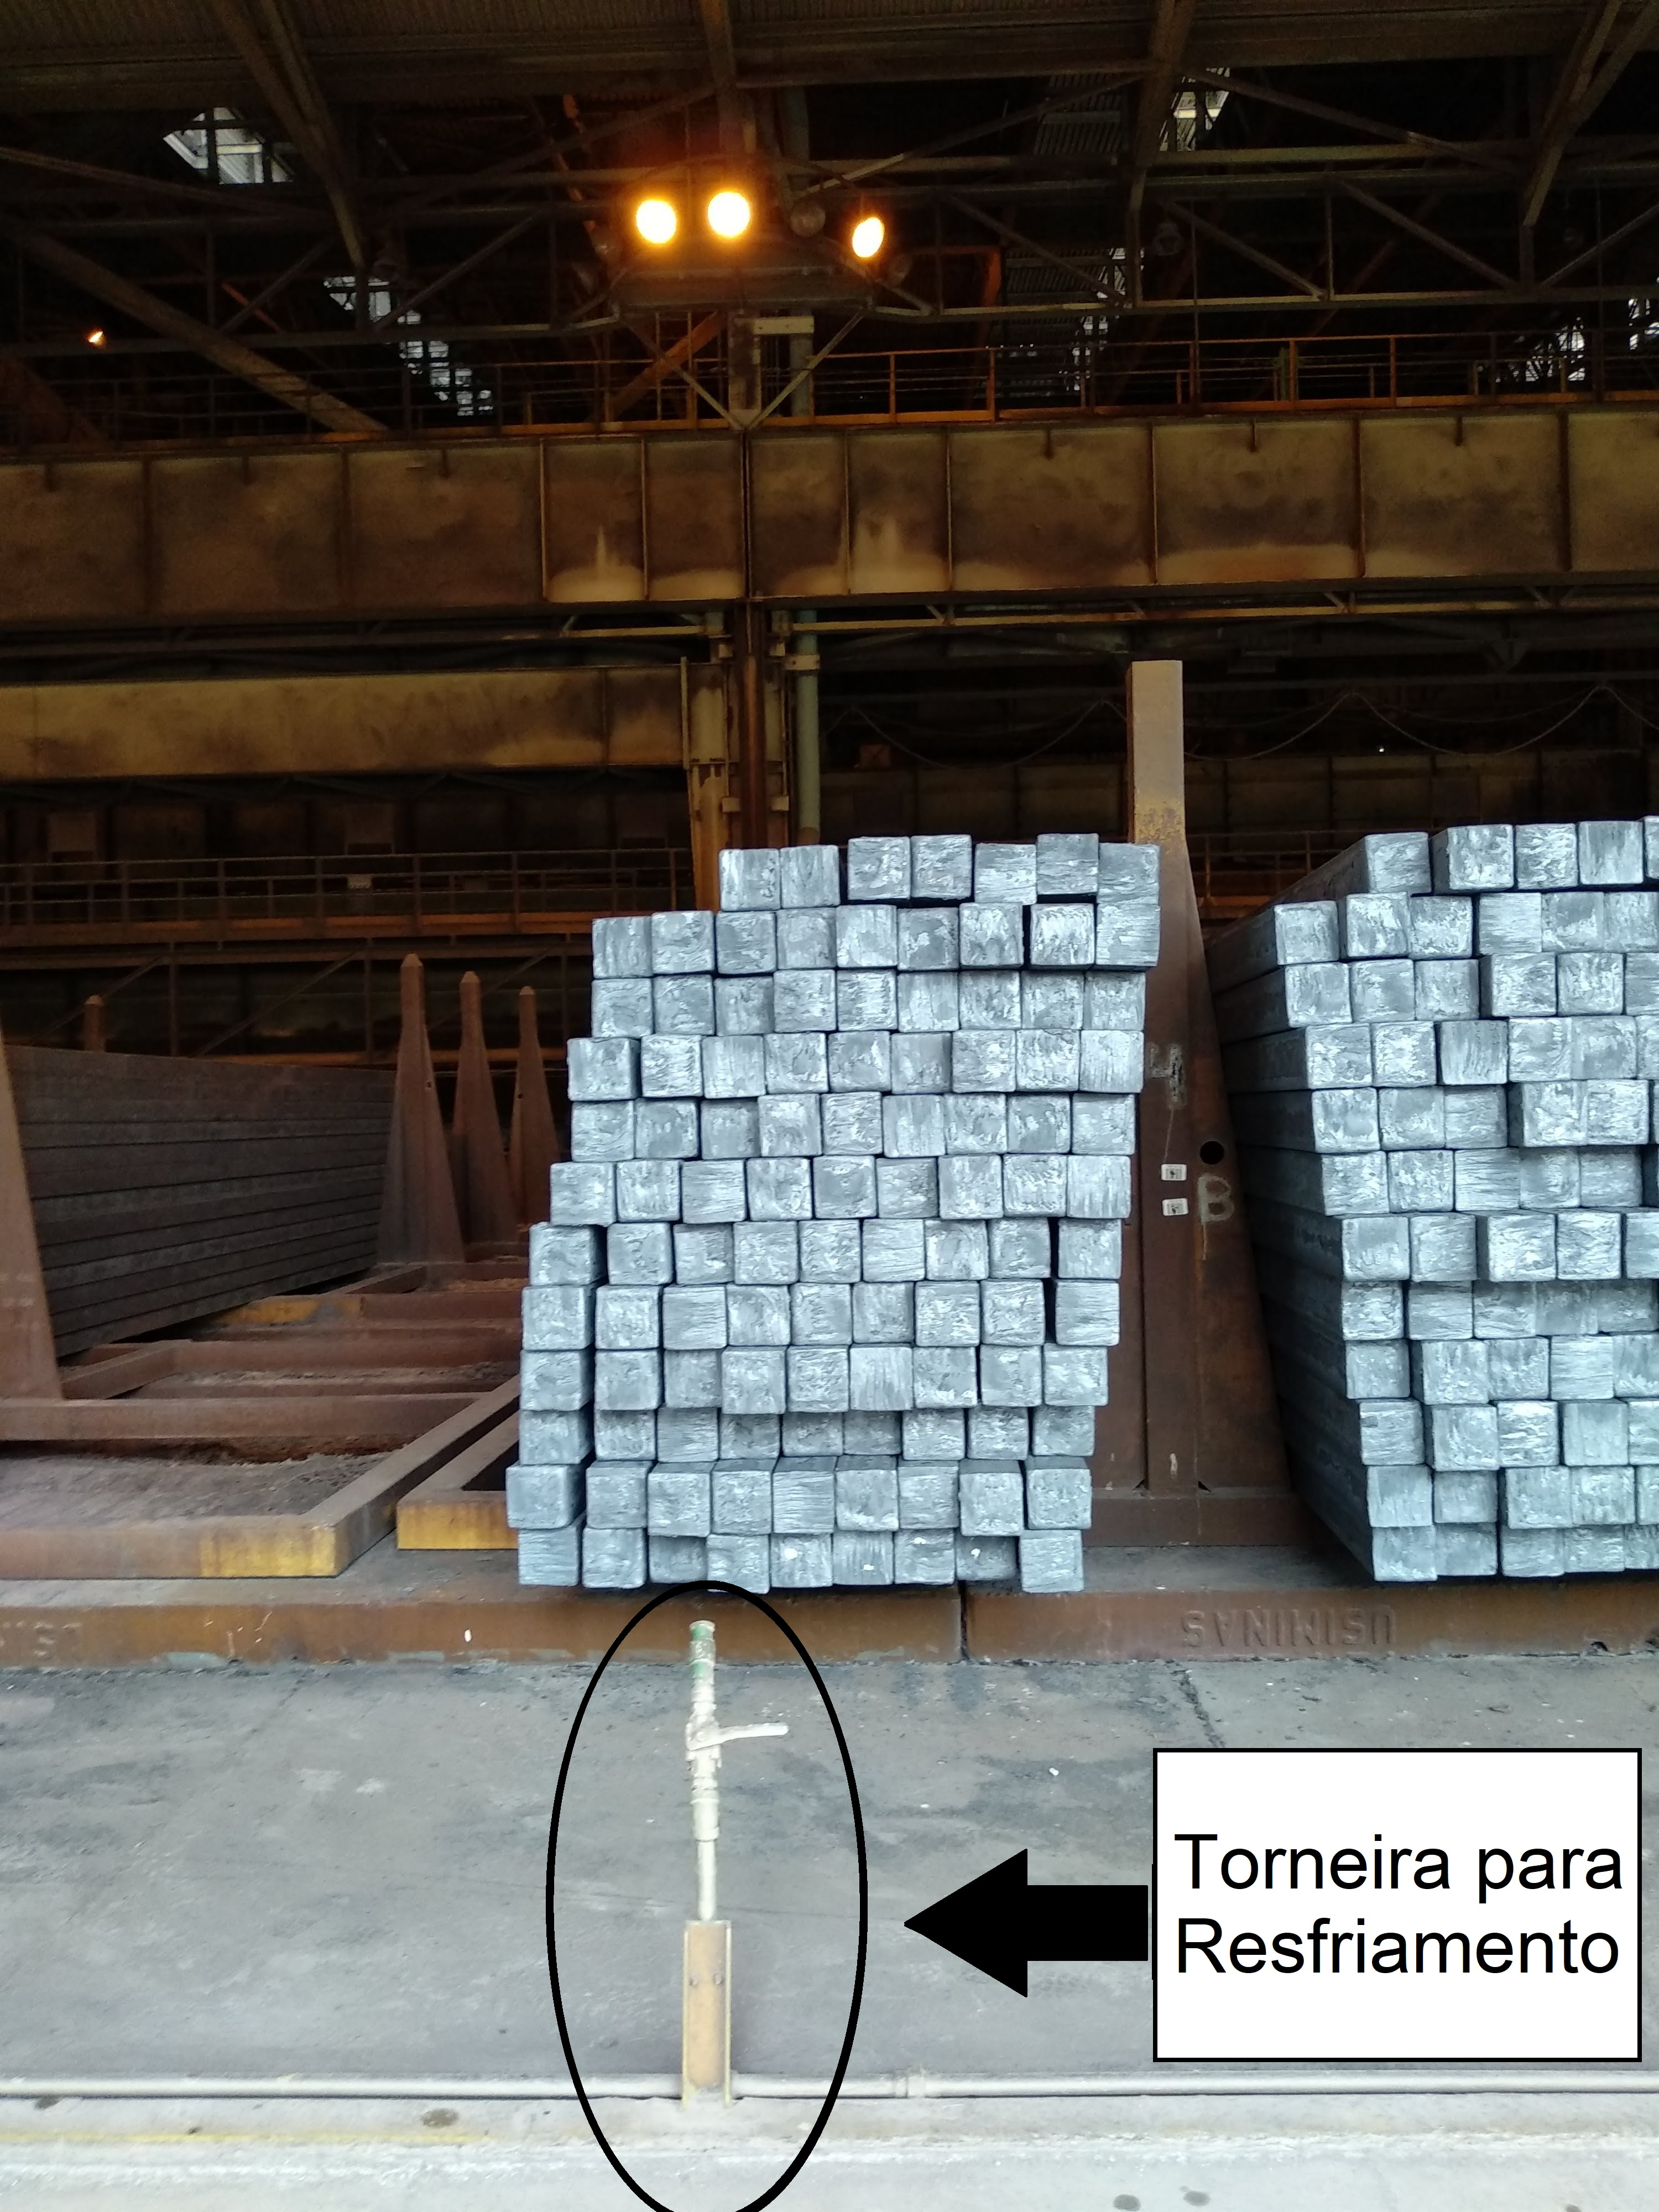
\includegraphics[width=0.5\linewidth]{figuras/Steel/despacho.jpg}
	\caption{Exemplo de Despacho: estoque de uma corrida}
	\label{fig:despacho}
\end{figure}

\begin{figure}[H]
	\centering
	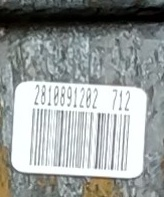
\includegraphics[width=0.25\linewidth]{figuras/Steel/barcode.jpg}
	\caption{Detalhe de uma etiqueta identificadora de um tarugo.} 
	\label{fig:barcode}
\end{figure}

A rotulação é importante pois evita a mistura de aço entre uma corrida e outra, viabiliza a rastreabilidade e identificação do aço em processos posteriores como, por exemplo, na laminação até o cliente final. A tabela \ref{tab:tag} mostra o que cada dígito da etiqueta significa.

\begin{table}[H]
	\centering
	\begin{tabular}{|l|l|}
		\hline
		\rowcolor[HTML]{ECF4FF} 
		\multicolumn{1}{|c|}{\cellcolor[HTML]{ECF4FF}Número} & \multicolumn{1}{c|}{\cellcolor[HTML]{ECF4FF}2810891202 712}\\ \hline
		28 & Número do convertedor que pode ser CV1 (27) ou CV2 (28).\\ \hline
		108912 & Adicionando o convertedor a este número, forma-se o número da corrida no qual: 
    		    \cr & CV2 = 2 e CV1 = 1, temos
    		    \cr & Número da corrida: 2108912\\ \hline
        02 & 02 é a rota que a panela passou no lingotamento. Ou seja, 02 = tarugo.\\ \hline
        712 & Número 7 é o veio que a peça foi lingotada e 12 o número da peça.\\ \hline
	\end{tabular}
	\caption{Significado dos dígitos da etiqueta de rotulação.}
	\label{tab:tag}
\end{table}

O número de identificação da etiqueta pode ser reconhecido pelos dígitos ou pelo código de barras através de um leitor de código de barras à \textit{laser}. Em cada etiqueta, o código de barras e os dígitos acima deste correspondem à mesma sequência numérica. Usualmente, a identificação ou leitura das etiquetas é feita por seres humanos e não por máquinas ou sistemas automáticos. Isto leva aos seguintes problemas:

\begin{enumerate}
	\item O processo é manual e demorado;
	\item O local em que a pilha de peças se encontra é perigoso devido ao fato de, a todo momento, uma ponte rolante estar trabalhando no mesmo local.
\end{enumerate}

\section{Revisão bibliográfica} 

Nesta seção é realizada a pesquisa na literatura a fim de investigar a relevância da automatização do processo de reconhecimento de imagem em indústrias siderúrgicas. Apresenta-se trabalhos semelhantes ao projeto proposto, bem como as dificuldades encontradas durante seus desenvolvimentos. 

Apesar do alto grau adaptativo e cognitivo, a identificação de imagens por uma pessoa pode gerar deficiências no processo por ser totalmente ligado à capacidade e estado do colaborador. O produto final do reconhecimento feito por um operador depende do nível de preparo, treinamento, capacidade visual e concentração, dentre outros fatores. \cite{refbib1} 
%
Além disto, estes parâmetros não são constantes, sofrendo alteração por motivos externos, como por exemplo, a iluminação ou cansaço. \cite{refbib2, refbib3}

No trabalho \citeauthor{ref1}, o autor trata da extração de números de gerenciamento de placas (SMNs) de imagens estáticas capturadas para automação do processo de fabricação de aço. Para impedir a mistura do produto em cada etapa da fabricação de aço, é essencial um sistema de reconhecimento automático das SMNs (Figura \ref{fig:SMN}). Além disso, o algoritmo de extração de SMNs com desempenho robusto é necessário porque afeta seriamente o desempenho de todo o sistema de reconhecimento. Contudo, resultados experimentais mostram que o algoritmo proposto é confiável. 


\begin{figure}[htbp]
	\centering
	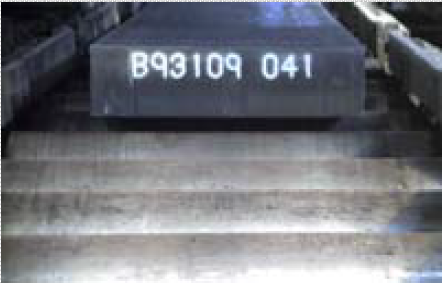
\includegraphics[width=0.5\linewidth]{figuras/Steel/SMN.png}
	\caption{Número de gerenciamento de placa}
	\label{fig:SMN}
\end{figure}


Em \citeonline{ref2}, os autores desenvolvem um sistema de reconhecimento em tempo real para caracteres gravados no material de placas e tarugos na planta de ferro fundido. 
%
Os tarugos normalmente são misturados no despacho, de modo que suas identificações são dificilmente tratáveis. Os caracteres dessa imagem do material podem ser marcados pelo uso de três tipos de métodos, como máquina de marcação automática, placa de marcação de modelo e escrita à mão. Para a aplicação do algoritmo de reconhecimento, desenvolveu-se um sistema de visão e instalou-se na linha de produção de placas e tarugos da planta de aço-ferro. Por meio do teste, confirmou-se que o sistema apresentou-se bom desempenho e alta taxa de reconhecimento: 97,6\% para placas e 98,6\% para tarugos.

O projeto \citeauthor{ref3}, descreve a implementação e análise de ferramentas propostas para reconhecimento de caracteres. Trata-se do problema de identificação de números de Ordem de Produção (OP) em peças de aço
(tarugos). O reconhecimento visa a automatização completa da LIT (linha de inspeção de tarugos). Com a possibilidade de identificação da OP, o sistema de reconhecimento deverá ser capaz de modificar as variáveis paramétricas da linha de inspeção de maneira a separar os tarugos para cada cliente, evitando-se problemas como mistura de peças e inspeções com parâmetros errados. São analisadas diversas imagens coletadas do processo real e o desempenho de cada etapa de processamento. Resultados das metodologias mostraram-se insatisfatórios, porém é aberta uma discussão a respeito da qualidade da imagem e o formato da estampagem dos caracteres no tarugo. São apontados itens críticos para mudança no processo e sugeridas modificações nas estratégias de maneira que se adequem melhor ao problema.



\section{Objetivos} 

O objetivo deste trabalho é desenvolver um sistema automático para o reconhecimento de etiquetas identificadoras em tarugos e uma interface para que o operador realize as conferências. 

Por meio de uma foto, o sistema será capaz de contar o número de etiquetas, identificar o código de barras e os números acima dele. Será criada uma aplicação web para que seja gerado, de forma automática, um relatório detalhado e facilitar a conferência por parte do operador.

\section{Organização do trabalho}

O presente trabalho está organizado em 4 capítulos. O atual apresenta o problema, possíveis soluções, e os objetivos propostos.
%
O Capítulo 2 apresenta a estrutura geral dos sistemas, das linguagens de programação, das bibliotecas, dos métodos e dos \textit{softwares} utilizados no projeto.
%
No Capítulo 3 são apresentados o desenvolvimento e os resultados deste trabalho. Explica-se também os experimentos realizados e códigos implementados.
%
No Capítulo 4 são abordadas as considerações finais do trabalho.